%% LyX 1.6.7 created this file.  For more info, see http://www.lyx.org/.
%% Do not edit unless you really know what you are doing.
\documentclass[brazil]{article}
\usepackage{ae,aecompl}
\usepackage[T1]{fontenc}
\usepackage[utf8]{inputenc}
\usepackage[a4paper]{geometry}
\geometry{verbose,lmargin=3cm,rmargin=3cm}
\setcounter{tocdepth}{0}
\usepackage{array}
\usepackage{float}
\usepackage{graphicx}

\makeatletter

%%%%%%%%%%%%%%%%%%%%%%%%%%%%%% LyX specific LaTeX commands.
%% Because html converters don't know tabularnewline
\providecommand{\tabularnewline}{\\}

%%%%%%%%%%%%%%%%%%%%%%%%%%%%%% User specified LaTeX commands.
%-%-%-%-%-%-%-%-%-%-%-%-%-%-%-%-%-%-%-%-%-%-%-%-%-%
% EE531: laboratório de Eletrônica Básica I       %  
% Experimento 2: Diodos                           %
% Data:20/08/2010                                 %
% Unicamp,Campinas,São Paulo,Brasil               % 
% Grupo:                                          %
%       - Daniel Lins Mattos                      %
%       - Raquel Mayumi Kawamoto                  %
%       - Tiago Chedraoui Silva                   % 
%-%-%-%-%-%-%-%-%-%-%-%-%-%-%-%-%-%-%-%-%-%-%-%-%-%
%\documentclass[letter]{article}  % formato impressao IC
 % formato impressao FEEC

%%% fontes %%%
% dá suporte para os termos na língua portuguesa do Brasi
% acentuação
\usepackage{ae}\usepackage{aecompl}\usepackage{aeguill}% pdfs mais bonitos =)

%%% outros %%%
\usepackage{multirow}\@ifundefined{definecolor}
 {\usepackage{color}}{}
\usepackage{indentfirst}% retira padrao americano de paragrafos
\usepackage{multicol}\usepackage[linkbordercolor={1 1 1},urlcolor=black,colorlinks=true]{hyperref}% links
\usepackage{subfig}

% circuito eletrico
\usepackage{electComp}\usetikzlibrary{decorations,decorations.pathmorphing,decorations.pathreplacing}
\usepackage{pstricks}\usepackage{boxdims}



\renewcommand{\thefigure}{\arabic{figure}}

\date{Novembro 12, 2010}
% Capa estilizada %
\newcommand*{\titleTMB}{\begingroup \centering \settowidth{\unitlength}{\LARGE EE531} {\large\scshape EE531 - Turma S}\\[0.2\baselineskip] \rule{11.0cm}{1.6pt}\vspace*{-\baselineskip}\vspace*{2pt} \rule{11.0cm}{0.4pt}\\[\baselineskip] {\LARGE  Amplificador operacional \\ com realimentação negativa}\\\vspace*{\baselineskip}  {\itshape Laboratório de Eletrônica Básica V - Segundo Semestre de 2010}\\ \rule{11.0cm}{0.4pt}\vspace*{-\baselineskip}\vspace{3.2pt} \rule{11.0cm}{1.6pt}\\[\baselineskip] {\large\scshape Professor: José Cândido Silveira Santos Filho}\par \vfill {\normalsize   \scshape 
    \begin{center} 
      \begin{tabular}{  l  l  p{5cm} } 
 	Daniel Lins Mattos & RA: 059915\\
        Raquel Mayumi Kawamoto & RA: 086003\\
        Tiago Chedraoui Silva  & RA: 082941\\
      \end{tabular} \end{center}
    \itshape 1 de outubro de 2010    }\\[\baselineskip] \vspace{3.2pt} \endgroup}

\makeatother

\usepackage{babel}

\begin{document}
\titleTMB \newpage{}

\begin{tabular}{c>{\centering}p{10cm}}
\hline 
Número pino & Descrição\tabularnewline
\hline
\hline 
1 & O pino 1 e o pino 5 costumam ser conectados a um resitor variável,
juntamente com a entrada negativa da alimentação, buscando equilibrar
as tensões da entrada.\tabularnewline
\hline 
2 & Entrada inversora\tabularnewline
\hline 
3 & Entrada não inversora\tabularnewline
\hline 
4 & Alimentação Negativa\tabularnewline
\hline 
5 & Off-set\tabularnewline
\hline 
6 & Tensão de saída\tabularnewline
\hline 
7 & Alimentação positiva\tabularnewline
\hline 
8 & Não conectado\tabularnewline
\hline
\end{tabular}

%
\begin{figure}[H]
\begin{centering}
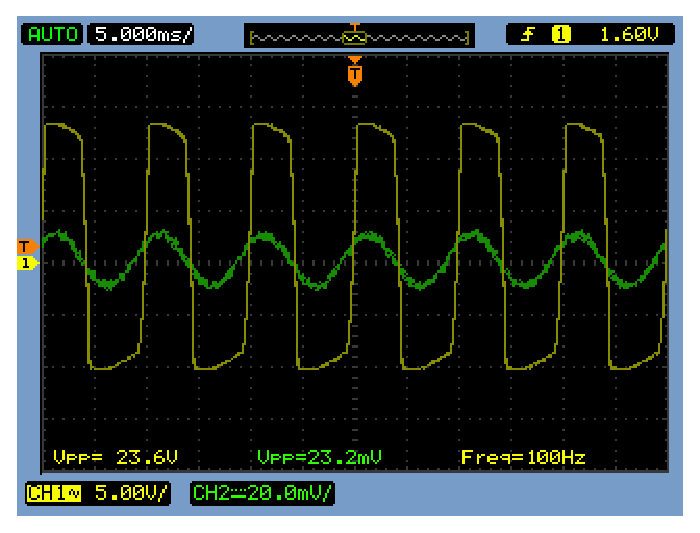
\includegraphics{figuras/31bck}
\par\end{centering}

\caption{}

\end{figure}


%
\begin{figure}[H]
\begin{centering}
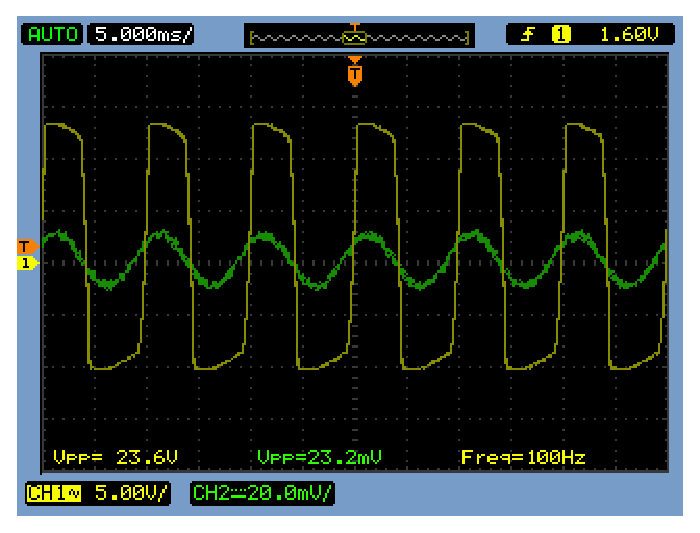
\includegraphics{figuras/31bck}
\par\end{centering}

\caption{}

\end{figure}
%
\begin{figure}[H]
\begin{centering}
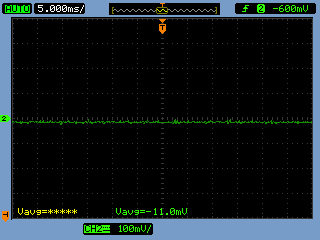
\includegraphics{figuras/382cres}
\par\end{centering}

\caption{}

\end{figure}
%
\begin{figure}[H]
\begin{centering}
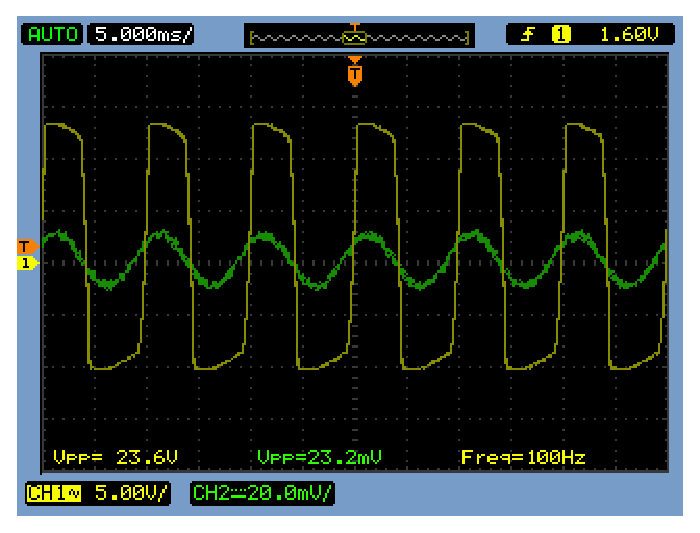
\includegraphics{figuras/31bck}
\par\end{centering}

\caption{}

\end{figure}


%
\begin{figure}[H]
\begin{centering}
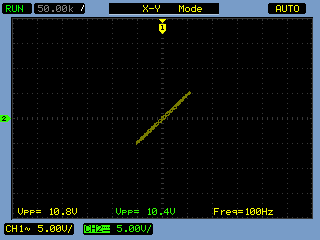
\includegraphics{figuras/35xy}
\par\end{centering}

\caption{}

\end{figure}
%
\begin{figure}[H]
\begin{centering}
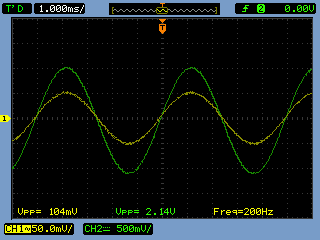
\includegraphics{figuras/37}
\par\end{centering}

\caption{}

\end{figure}
%
\begin{figure}[H]
\begin{centering}
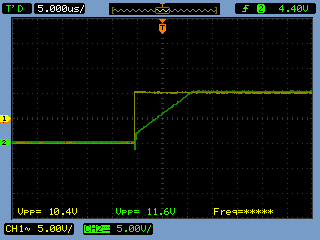
\includegraphics{figuras/36}
\par\end{centering}

\caption{}

\end{figure}


%
\begin{figure}[H]
\begin{centering}
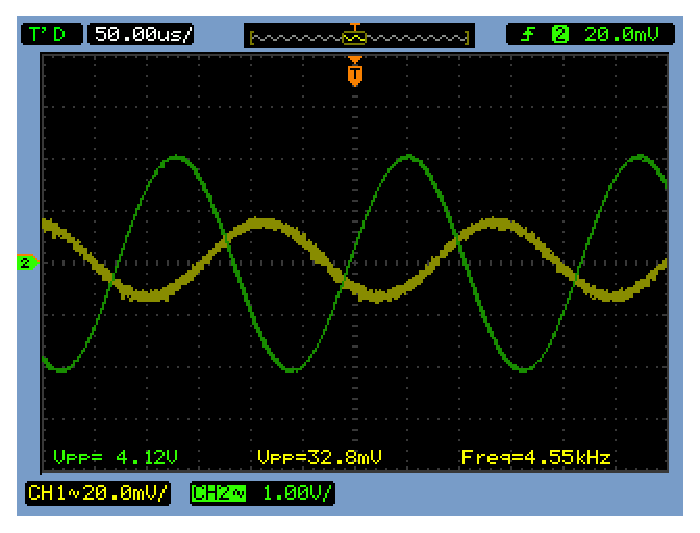
\includegraphics{figuras/311fh}
\par\end{centering}

\caption{}

\end{figure}
%
\begin{figure}[H]
\begin{centering}
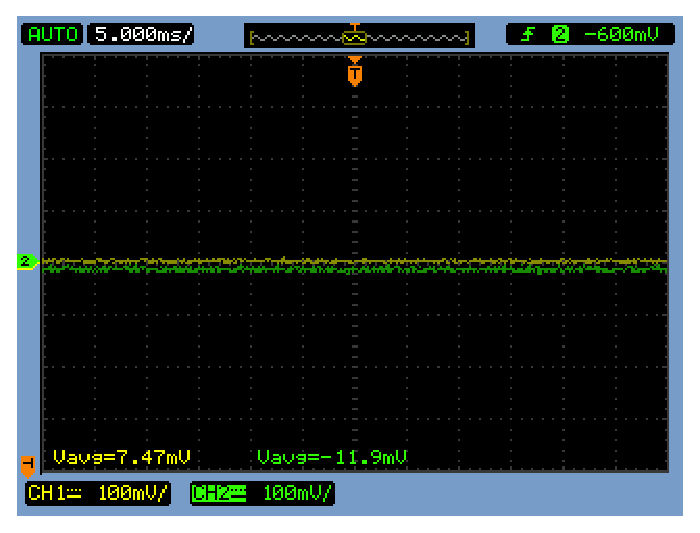
\includegraphics{figuras/382cr}
\par\end{centering}

\caption{}

\end{figure}
%
\begin{figure}[H]
\begin{centering}
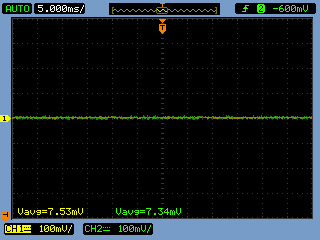
\includegraphics{figuras/39}
\par\end{centering}

\caption{}

\end{figure}
%
\begin{figure}[H]
\begin{centering}
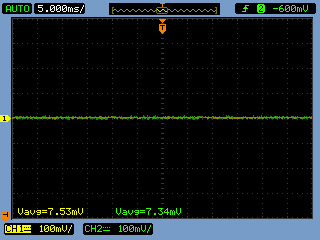
\includegraphics{figuras/39}
\par\end{centering}

\caption{}

\end{figure}
%
\begin{figure}[H]
\begin{centering}
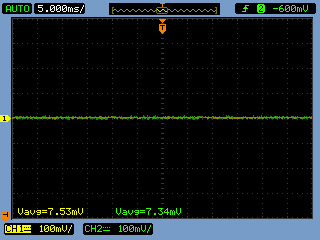
\includegraphics{figuras/39}
\par\end{centering}

\caption{}

\end{figure}
%
\begin{figure}[H]
\begin{centering}
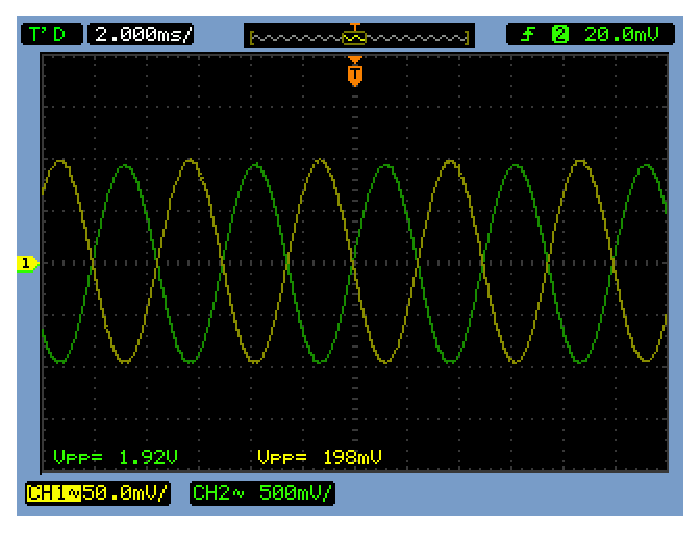
\includegraphics{figuras/310}
\par\end{centering}

\caption{}

\end{figure}

\end{document}
